% Erstellt von Maximilian Nöthe, <maximilian.noethe@tu-dortmund.de>
% ausgelegt für lualatex und Biblatex mit biber

% Kompilieren mit 
% lualatex dateiname.tex
% biber dateiname.bcf
% lualatex dateiname.tex
% lualatex dateiname.tex
% oder einfach mit:
% make

\documentclass[
  tucolor,
  BCOR=12mm,     % 12mm binding corrections, adjust to fit your binding
  parskip=half,  % new paragraphs start with half line vertical space
  open=any,      % chapters start on both odd and even pages
  cleardoublepage=plain,  % no header/footer on blank pages
]{tudothesis}


% Warning, if another latex run is needed
\usepackage[aux]{rerunfilecheck}

% just list chapters and sections in the toc, not subsections or smaller
\setcounter{tocdepth}{1}

%------------------------------------------------------------------------------
%------------------------------ Sprache und Schrift: --------------------------
%------------------------------------------------------------------------------
\usepackage{fontspec}
\defaultfontfeatures{Ligatures=TeX}  % -- becomes en-dash etc.

% german language
\usepackage{polyglossia}
\setdefaultlanguage{english}

% for english abstract and english titles in the toc
%\setotherlanguages{english}

% intelligent quotation marks, language and nesting sensitive
\usepackage[autostyle]{csquotes}

% microtypographical features, makes the text look nicer on the small scale
\usepackage{microtype}

%------------------------------------------------------------------------------
%------------------------ Für die Matheumgebung--------------------------------
%------------------------------------------------------------------------------

\usepackage{amsmath}
\usepackage{amssymb}
\usepackage{mathtools}
\usepackage{slashed}

% Enable Unicode-Math and follow the ISO-Standards for typesetting math
\usepackage[
  math-style=ISO,
  bold-style=ISO,
  sans-style=italic,
  nabla=upright,
  partial=upright,
]{unicode-math}
\setmathfont{Latin Modern Math}

% nice, small fracs for the text with \sfrac{}{}
\usepackage{xfrac}  


%------------------------------------------------------------------------------
%---------------------------- Numbers and Units -------------------------------
%------------------------------------------------------------------------------

\usepackage[
  locale=DE,
  separate-uncertainty=true,
  per-mode=symbol-or-fraction,
  output-decimal-marker=., % . statt , für Dezimalzahlen
]{siunitx}
\sisetup{math-micro=\text{µ},text-micro=µ}

%------------------------------------------------------------------------------
%-------------------------------- tables  -------------------------------------
%------------------------------------------------------------------------------

\usepackage{booktabs}       % stellt \toprule, \midrule, \bottomrule

%------------------------------------------------------------------------------
%-------------------------------- graphics -------------------------------------
%------------------------------------------------------------------------------

\usepackage{graphicx}
\usepackage{grffile}
\usepackage{tikz}
\usetikzlibrary{decorations}
\usetikzlibrary{decorations.markings}
\usetikzlibrary{decorations.pathmorphing}
\usetikzlibrary{arrows.meta}


% allow figures to be placed in the running text by default:
\usepackage{scrhack}
\usepackage{float}
\floatplacement{figure}{htbp}
\floatplacement{table}{htbp}

% keep figures and tables in the section
\usepackage[section, below]{placeins}


%------------------------------------------------------------------------------
%---------------------- customize list environments ---------------------------
%------------------------------------------------------------------------------

\usepackage{enumitem}

%------------------------------------------------------------------------------
%------------------------------ Bibliographie ---------------------------------
%------------------------------------------------------------------------------

\usepackage[
  backend=biber,   % use modern biber backend
  autolang=hyphen, % load hyphenation rules for if language of bibentry is not
  sorting=none,    % german, has to be loaded with \setotherlanguages
  maxbibnames=4,   % in the references.bib use langid={en} for english sources
]{biblatex}
\addbibresource{references.bib}  % die Bibliographie einbinden
\DefineBibliographyStrings{english}{andothers = {{et\,al\adddot}}} 

%------------------------------------------------------------------------------
%------------------------------ Sonstiges: ------------------------------------
%------------------------------------------------------------------------------

\usepackage[pdfusetitle,unicode,linkbordercolor=tugreen]{hyperref}
\usepackage{bookmark}
\usepackage[shortcuts]{extdash}
\usepackage[
	hide
	]{todo}

%------------------------------------------------------------------------------
%-------------------------    Angaben zur Arbeit   ----------------------------
%------------------------------------------------------------------------------

\author{Anja Beck}
\title{Flavour Mixing Effects in the Direct Detection of Dark Matter}
\date{2017}
\birthplace{Kempten (Allgäu)}
\chair{Lehrstuhl für Theoretische Physik IV}
\division{Fakultät Physik}
\thesisclass{Bachelor of Science}
\submissiondate{17. Juli 2017}
\firstcorrector{Jun.-Prof.~Dr.~Joachim Brod}
\secondcorrector{Prof.~Dr.~Heinrich Päs}

% tu logo on top of the titlepage
\titlehead{
\includegraphics[height=1.5cm]{logos/tu-logo.pdf}}

\begin{document}
\frontmatter
%\input{content/hints.tex}
\maketitle

% Gutachterseite
\makecorrectorpage

% hier beginnt der Vorspann, nummeriert in römischen Zahlen
\thispagestyle{plain}
\section*{Abstract}
Quark flavour mixing is often neglected because of its small effects. But since dark matter only interacts weakly with baryonic matter, these tiny effects might be of importance for direct detection. This thesis examines whether flavour mixing was rightfully neglected by Altmannshofer et. al. in the discussion of a new interaction \cite{Z}. Therefore, we expand an existing framework for dark matter direct detection with the CKM mixing matrix. In the second part of this thesis, we present the new interaction, that was originally proposed to explain anomalies in the decay $B\rightarrow Kl\bar{l}$, but also makes predictions about the direct detection of dark matter. However, when treating dark matter cross sections, this new set-up ignores flavour mixing effects. Thus, we compare those new cross sections with cross sections obtained with flavour mixing and conclude that, in this case, flavour mixing was rightfully neglected.
\cleardoublepage
\tableofcontents

\mainmatter
% Hier beginnt der Inhalt mit Seite 1 in arabischen Ziffern
\chapter{Introduction}
We will take a look at the effects of the flavour mixing mechanism on the direct detection of dark matter. Therefore we expand an existing formalism for dark matter direct detection with the CKM matrix. Afterwards we present a new interaction proposed to explain anomalies in the decay $B\rightarrow Kl\bar{l}$ that also makes predictions about the direct detection of dark matter. Finally, we compare these predictions with the direct detection cross sections that respect flavour mixing.

Direct detection means detecting dark matter directly through interaction with a nucleus, in contrary to indirect detection, which means measuring secondary products of dark matter annihilation or dark matter decay.

\todo{Irgendwo muss noch kurz auf dunkle Materie eingegangen werden. Als Einleitung wären daher auch Detection Experimente gut. Evtl. hier direct vs indirect erklären.}


\begin{figure}
	\centering
	\begin{tikzpicture}
\tikzstyle{centerArrow}=[decoration={
    markings,
    mark=at position 0.5 with {\fill (2pt,0)--(-2pt,2.31pt)--(-2pt,-2.31pt)--cycle;}}]
\begin{scope}
\def\xmove{2.5}
\def\ymove{1.25}
\def\centerSize{0.15}
\node [fill, circle,inner sep=\centerSize cm] (tCenter)  {};
\node (upperLeft) at (-\xmove,\ymove) {$\chi$};
\node (upperRight) at (\xmove,\ymove) {$\chi$};
\node (lowerLeft) at (-\xmove,-\ymove) {$N$};
\node (lowerRight) at (\xmove,-\ymove) {$N$};
\draw [centerArrow,postaction={decorate}]  (upperLeft) -- (tCenter) ;
\draw [centerArrow,postaction={decorate}]  (lowerLeft) -- (tCenter) ;
\draw [centerArrow,postaction={decorate}]  (tCenter) -- (upperRight) ;
\draw [centerArrow,postaction={decorate}]  (tCenter) -- (lowerRight) ;
\end{scope}
\end{tikzpicture}
	\caption{Direct detection}
	\label{fig:DirectDetection}
\end{figure}
\chapter{The Flavour Mixing Mechanism}
The origins of flavour mixing go back to the 1960s, when the Italian physicist Nicola Cabibbo resolved anomalies in data of weak interactions by proposing a flavour mixing of left-handed down-type quarks. Later in 1973, Kobayaski and Maskawa extended this idea to three quark generations to explain CP violation \cite{Griffiths}. On a mathematical level, quark flavour mixing arises from the fact that the fermion mass eigenstates do not necessarily coincide with the flavour eigenstates. In the course of this chapter, we first derive how the Higgs mechanism gives mass to particles and second take a look at fermion masses and why this leads to flavour mixing. The following calculations are based on the outlines in the textbook by Peskin and Schroeder \cite[Chapter 20]{Peskin} and the theoretical discussion of CP violation in \mbox{\cite[Chapter 1.2.1]{Tevatron}.}
\section{The Higgs Mechanism}
We consider a complex scalar field $\Phi$ that interacts with itself through a potential
\begin{align}
	V(\Phi) = -\mu^2\Phi^\dagger\Phi + \frac{\lambda}{2}(\Phi^\dagger\Phi)^2 \ , \quad \mu^2 > 0 \ .
\end{align}
If $\lambda>0$, there are two minima of this potential. They occur at
\begin{align}
	\langle\Phi\rangle =  \pm\sqrt{\frac{\mu^2}{\lambda}} \ .
\end{align}
This is the vacuum expectation value of $\Phi$.

We add a $SU(2)$ gauge field coupled to $\Phi$, so $\Phi$ is a doublet $(\Phi_1,\Phi_2)$ with covariant derivative
\begin{align}
	D_\mu\Phi = (\partial_\mu - ig\sum_{a=1}^3A_\mu^a\tau^a)\Phi \ ,
\end{align}
where $\tau^a$ are the generators of $SU(2)$. In this case there is an infinite number of vacuum expectation values for $\Phi$ arranged in a circle. We are free to choose one and make the simple choice
\begin{align}\label{eq:vev}
	\langle\Phi\rangle = \frac{1}{\sqrt{2}}\begin{pmatrix} 0 \\ v \end{pmatrix} \ , \qquad v = \sqrt{\frac{2\mu^2}{\lambda}} \ .
\end{align}
Note that by choosing one vacuum value, we break the symmetry.


The kinetic energy of $\Phi$ is
\begin{align}
	(D_\mu\Phi)^2 = &\frac{1}{2}(\partial_\mu v)(\partial^\mu v)\notag \\
	- &ig(\partial^\mu\begin{pmatrix} 0 & v \end{pmatrix}) \left(\sum_{a=1}^3A_\mu^a\tau^a\begin{pmatrix} 0 \\ v \end{pmatrix}\right)\notag \\
	- &\frac{1}{2}g^2\begin{pmatrix} 0 & v \end{pmatrix}\sum_{a,b=1}^{3}\tau^a\tau^b\begin{pmatrix} 0 \\ v \end{pmatrix}A_\mu^aA^{b\mu} \ .
\end{align}
Using the relation $\{\tau^a,\tau^b\}=\sfrac{1}{2}\cdot\delta_{ab}$, we can simplify the last expression to get
\begin{align}
	- \frac{1}{2}g^2\begin{pmatrix} 0 & v \end{pmatrix}\sum_{a,b=1}^{3}\tau^a\tau^b\begin{pmatrix} 0 \\ v \end{pmatrix}A_\mu^aA^{b\mu} &= - \frac{g^2v^2}{8}\sum_{a=1}^{3}A_\mu^aA^{a\mu} \ ,
\end{align}
which is a mass term $\mathcal{L}_m = -\frac{1}{2}m_A^2A_\mu A^\mu$ that assigns the mass $m_A = \frac{gv}{2}$ to all three gauge bosons. By expanding the system with an additional $U(1)$ symmetry, the kinetic energy would again provide three gauge boson masses, leaving the fourth gauge boson massless. The massive bosons can be identified as $W^\pm,Z^0$ and the massless as the photon.


The scalar field $\Phi$ is usually called Higgs boson. Obtaining particle mass terms in the kinetic energy of the Higgs, is, unsurprisingly, referred to as the Higgs mechanism. 
%
%
%We expand the system with an additional $U(1)$ symmetry with gauge boson $B$. The field $\Phi$ has a charge $Y_\Phi$ under $U(1)$. The new covariant derivative is
%\begin{align}
%	D_\mu\Phi = \left(\partial_\mu - ig\sum_{a=1}^3A_\mu^a\tau^2 - iY_\Phi g'B_\mu\right)\Phi \ .
%\end{align}
%Again, we examine the kinetic term
%\begin{align}
%	(D_\mu\Phi)^2 = &\frac{1}{2}(\partial_\mu v)(\partial^\mu v)\notag \\
%	- &\frac{1}{2}i\left(\partial^\mu\begin{pmatrix} 0 & v \end{pmatrix}\right) \left(g\sum_{a=1}^3A_\mu^a\tau^2 + Y_\Phi g'B_\mu\right)\begin{pmatrix} 0 \\ v \end{pmatrix}\notag \\
%	- &\frac{1}{2}\begin{pmatrix} 0 & v \end{pmatrix}
%	\left(g^2\sum_{a,b=1}^3A_\mu^aA^{b\mu}\tau^a\tau^b + 2gg'Y_\Phi\sum_{a=1}^3A_\mu^a\tau^aB^\mu + Y_\Phi^2g'^2B_\mu B^\mu\right)
%	\begin{pmatrix} 0 \\ v \end{pmatrix}
%\end{align}
%Using $\{\tau^a,\tau^b\}=\sfrac{1}{2}\cdot\delta_{ab}$ and replacing $\tau^a=\sfrac{\sigma^a}{2}$, we find for the last term
%\begin{align}
%	\mathcal{L}^{(\text{mass})} &= - \frac{v^2}{2}\left(g^2\frac{1}{4}\sum_{a=1}^3A_\mu^aA^{a\mu} + Y_\Phi^2g'^2B_\mu B^\mu - gg'Y_\Phi B^\mu A_\mu^3\right)\notag \\
%	&= - \frac{1}{2}\frac{v^2}{4}\left(g^2A_\mu^1A^{1\mu} + g^2A_\mu^2A^{2\mu} + (gA_\mu^3 - 2g'Y_\Phi B_\mu)^2\right)\notag \\
%	&= - \frac{1}{2}\frac{v^2}{4}\left(g^22W^+W^- + (g^2+4g'^2Y_\Phi^2)Z_0^2\right) \ .
%\end{align}
%Here we identified the known vector bosons
%\begin{align}
%	W_\mu^\pm &= \frac{1}{\sqrt{2}}(A_\mu^1\mp iA_\mu^2) \ , &&\quad &m_W &= \frac{v}{2}g \notag \\
%	Z_\mu^0 &= \frac{1}{\sqrt{g^2+4g'^2Y_\Phi^2}}(gA_\mu^3 - 2g'Y_\Phi B_\mu) \ , &&\quad &m_Z &= \frac{v}{2}\sqrt{g^2+4g'^2Y_\Phi^2}
%\end{align}
%as mass eigenstates of the gauge bosons.
%
%
%Since we are in a $SU(2)\times U(1)$ symmetry, there has to be a fourth gauge boson. As we have just derived, it is massless. We renounce giving an elaborate explanation for this, but we want to give a motivation. Therefore we need to remember that the masses arise through choosing a vacuum expectation value for $\Phi$ and thereby breaking the $SU(2)$ symmetry. Looking at the gauge transformation of $\Phi$
%\begin{align}
%	\Phi\rightarrow e^{i\sum_{a=1}^3\alpha^a\tau^a}e^{i\beta Y_\Phi}\Phi \ ,
%\end{align}
%we find that the choice $\alpha^1=\alpha^2=0$, $\alpha^3 = 2\beta Y_\Phi$ leaves the vacuum expectation value unchanged. Thus, parts of the symmetry are conserved and keep one gauge boson from acquiring mass. The fourth gauge boson is the photon, and it is orthogonal to $Z_\mu^0$:
%\begin{align}
%	A_\mu = \frac{1}{\sqrt{g^2 + 2g'^2Y_\Phi^2}}(2g'Y_\Phi A^3_\mu + gB_\mu) \ .
%\end{align}

\section{Fermion Masses and Flavour Mixing}
Hereafter, we describe how the standard model fermions get their masses and how this leads to quark flavour mixing. But beforehand, we introduce the notation used in this and the following chapters. The leptons and quark chiral particle multiplets are
\begin{align}
	E_R &= (e_R,\mu_R,\tau_R) \ , &&\quad &Y_E &= -2 \ ; \\
	L_L &= \left(\begin{pmatrix} \nu_e \\ e \end{pmatrix}_L,
	\begin{pmatrix} \nu_\mu \\ \mu \end{pmatrix}_L,
	\begin{pmatrix} \nu_\tau \\ \tau \end{pmatrix}_L\right) \ , &&\quad &Y_L &= -1 \ ; \\
	U_R &= (u_R,c_R,t_R) \ , &&\quad &Y_U &= \frac{4}{3} \ ; \\
	D_R &= (d_R,s_R,b_R) \ , &&\quad &Y_D &= -\frac{2}{3} \ ; \\
	Q_L &= \left(\begin{pmatrix} u \\ d \end{pmatrix}_L,
	\begin{pmatrix} c \\ s \end{pmatrix}_L,
	\begin{pmatrix} t \\ b \end{pmatrix}_L\right) \ , &&\quad &Y_Q &= \frac{1}{3} \ ;
\end{align}
where the hypercharge $Y$ is given. It is related to the electric charge $Q$ and the third component of the weak isospin $I_3$ through the Gell-Mann-Nishijima formula \cite[Chapter 10.7]{Griffiths}
\begin{align}\label{eq:GellMann}
	Q = \frac{Y}{2} + I_3 \ .
\end{align}
The right-handed particles are singlets under $SU(2)$ and therefore $I^{(r.h.)}_3=0$. We later also use the left-handed components $E_L = (e_L,\mu_L,\tau_L)$, $D_L = (d_L,s_L,b_L)$, and $U_L = (u_L,c_L,t_L)$.


The electroweak interaction lagrangian for the standard model fermions is
\begin{align}\label{eq:LFermion}
%	\mathcal{L}^{(\text{int})} = &\sum_{i=1}^{3}\bar{E}_R^i(i\slashed{\partial}-g_1Y_E\slashed{B})E_R^i + \bar{D}_R^i(i\slashed{\partial}-g_1Y_D\slashed{B})D_R^i + \bar{U}_R^i(i\slashed{\partial}-g_1Y_U\slashed{B})U_R^i \notag \\
%	+ &\sum_{i=1}^{3}\bar{L}_L^i(i\slashed{\partial}-g_1Y_L\slashed{B}-g_2\slashed{A})L_L^i + \bar{Q}_L^i(i\slashed{\partial}-g_1Y_Q\slashed{B}-g_2\slashed{A})Q_L^i \ ,
	\mathcal{L}^{(\text{int})} = &\bar{E}_R\gamma^\mu(i\partial_\mu-g_1Y_EB_\mu)E_R + \bar{L}_L\gamma^\mu(i\partial_\mu-g_1Y_LB_\mu-g_2\sum_{a=1}^{3}A_\mu^a\tau^a)L_L \notag \\
	+ &\bar{D}_R\gamma^\mu(i\partial_\mu-g_1Y_DB_\mu)D_R + \bar{U}_R\gamma^\mu(i\partial_\mu-g_1Y_UB_\mu)U_R \notag \\
	+ &\bar{Q}_L\gamma^\mu(i\partial_\mu-g_1Y_QB_\mu-g_2\sum_{a=1}^{3}A_\mu^a\tau^a)Q_L \ ,
\end{align}
where $B_\mu, A_\mu^a$ are the gauge bosons corresponding to $U(1)_Y\times SU(2)$. The coupling constants are $g_1$ and $g_2$, and the $\tau^a$ are again the $SU(2)$ generators. This lagrangian describes massless particles. In order to get a fermion mass term, one has to couple the left- and right-handed part of a particle. Since a direct coupling between a $SU(2)$ singlet and a $SU(2)$ doublet violates gauge invariance, a connecting field is necessary. To preserve invariance under Lorentz, $U(1)_Y$, and $SU(2)$ transformations, this field must have spin 0, hypercharge $Y=\sfrac{1}{2}$, and be a doublet. We identify this field with $\Phi$ from the previous chapter and write down the mass terms for the fermions
\begin{align}
%	\mathcal{L}^{(\text{mass})} = -\sum_{i,j=1}^{3}\left[\lambda^e_{ij} \bar{L}_L^i\Phi E_R^j  + \lambda_{ij}^d\bar{Q}_L^i\Phi D_R^j + \lambda_{ij}^u\sum_{a,b=1}^{2}\epsilon_{ab}\bar{Q}_{La}^{i}\Phi_b^\dagger U_R^j + \text{h.c.}\right] \ ,
	\mathcal{L}^{(\text{mass})} = -\left[\bar{L}_L\Phi\lambda^e  E_R  + \bar{Q}_L\Phi\lambda^d D_R + \bar{Q}_Li\sigma^2\Phi^\dagger\lambda^u U_R + \text{h.c.}\right] \ ,
\end{align}
with complex matrix coupling constants $\lambda^e,\lambda^d,\lambda^u$. Replacing $\Phi$ with its vacuum expectation value \eqref{eq:vev2} gives
\begin{align}\label{eq:LMass}
%	\mathcal{L}^{(\text{mass})} = -\frac{v}{\sqrt{2}}\sum_{i,j=1}^{3}\left[\lambda^e_{ij} \bar{E}_L^i E_R^j  + \lambda_{ij}^d\bar{D}_L^i D_R^j + \lambda_{ij}^u\bar{U}_L^{i} U_R^j + \text{h.c.}\right] \ ,
	\mathcal{L}^{(\text{mass})} = -\frac{v}{\sqrt{2}}\left[ \bar{E}_L\lambda^e E_R  + \bar{D}_L \lambda^dD_R + \bar{U}_L\lambda^u U_R + \text{h.c.}\right] \ .
\end{align}



The interaction lagrangian $\mathcal{L}^{(\text{int})}$ (see \eqref{eq:LFermion}) is invariant under the unitary transformations
\begin{align}
	E_L &\rightarrow S_eE_L \ , && &E_R &\rightarrow R_eE_R \ , \\
	U_L &\rightarrow S_uU_L \ , && &U_R &\rightarrow R_uU_R \ , \\
	D_L &\rightarrow S_dD_L \ , && &D_R &\rightarrow R_dD_R \ .
\end{align}
Thus, we can diagonalize the interactions in \eqref{eq:LMass}, using these transformations. The diagonal lepton coupling is $\tilde{\lambda}^e = S_e\lambda^eR_e^\dagger$ and parametrizes the lepton masses
\begin{align}
	m_e = \frac{v}{\sqrt{2}}\tilde{\lambda}_{11}^e \ , \quad m_\mu = \frac{v}{\sqrt{2}}\tilde{\lambda}_{22}^e \ , \quad m_\tau = \frac{v}{\sqrt{2}}\tilde{\lambda}_{33}^e \ .
\end{align}
The diagonal coupling for up-type quarks is $\tilde{\lambda}^u = S_u\lambda^uR_u^\dagger$, giving the corresponding masses
\begin{align}
	m_u = \frac{v}{\sqrt{2}}\tilde{\lambda}_{11}^u \ , \quad m_c = \frac{v}{\sqrt{2}}\tilde{\lambda}_{22}^u \ , \quad m_t = \frac{v}{\sqrt{2}}\tilde{\lambda}_{33}^u \ .
\end{align}
The transformed coupling of the down-type quarks is $\tilde{\lambda}^d = S_d\lambda^dR_d^\dagger$, leading to the down-type masses
\begin{align}
	m_d = \frac{v}{\sqrt{2}}\tilde{\lambda}_{11}^d \ , \quad m_s = \frac{v}{\sqrt{2}}\tilde{\lambda}_{22}^d \ , \quad m_b = \frac{v}{\sqrt{2}}\tilde{\lambda}_{33}^d \ .
\end{align}


The transformed particle multiplets are now mass eigenstates. But when looking at couplings of up- and down-type quarks, e. g. the current
\begin{align}
	\bar{U}_L\gamma^\mu D_L \ ,
\end{align}
the unitary transformations change the interaction to
\begin{align}
	\bar{U}_L\gamma^\mu S_u^\dagger S_d D_L \ ,
\end{align}
where we identify the CKM matrix $V=S_u^\dagger S_d$. Because $S_u,S_d$ are already determined by the diagonalizations above, the CKM matrix is not equal to the identity matrix in general. In fact, $V$ alters left-handed currents measurably. The most recent data by the Particle Data Group determines the parameters of the Wolfenstein parametrization
\begin{align}
	V = \begin{pmatrix}
	1-\frac{\lambda^2}{2} & \lambda & A\lambda^3(\rho-i\eta) \\
	-\lambda & 1-\frac{\lambda^2}{2} & A\lambda^2 \\
	A\lambda^3(1-\rho-i\eta) & -A\lambda^2 & 1
	\end{pmatrix}
\end{align}
to be (see \cite[Chapter 12]{PDG})
\begin{align}\label{eq:Wolf}
	\lambda &= \SI{0.22496(48)}{} \ , && &A &= \SI{0.823(13)}{} \ , \notag \\
	\rho &= \SI{0.141(19)}{} \ , && &\eta &= \SI{0.349(12)}{} \ .\footnotemark
\end{align}
\footnotetext{The Particle Data Group actually suggests two different sets of parameters obtained by two different methods. We choose one arbitrarily, because they only differ in the second decimal position, which does not make any difference in our calculations later.}
\chapter{Introduction of the Flavour Mixing into an Existing Formalism\label{sec:formalism}}
In this chapter we incorporate flavour mixing into an existing formalism. We use the model described in \cite{ChiralEFT}. It provides a framework to calculate cross sections for the direct detection of dark matter. The model is based on a set of dimension-five, -six, and -seven operators. We restrict our calculations to the dimension-six operators, which are
\begin{align}\label{eq:normal}
	R_{1,q} &= (\bar{\chi}_0\gamma_\mu\chi_0)(\bar{q}\gamma^\mu q) \ , && &R_{3,q} &= (\bar{\chi}_0\gamma_\mu\chi_0)(\bar{q}\gamma^\mu\gamma_5q) \ , \notag \\
	R_{2,q} &= (\bar{\chi}_0\gamma_\mu\gamma_5\chi_0)(\bar{q}\gamma^\mu q) \ , &&	&R_{4,q} &= (\bar{\chi}_0\gamma_\mu\gamma_5\chi_0)(\bar{q}\gamma^\mu\gamma_5q) \ .
\end{align}
Here $q=(u,d,c,s,t,b)$ is a quark and $\chi_0$ is the component of the weak dark matter mutliplet that has no electric charge.


Since the CKM mixing only applies to the left-handed down-type quarks, we need to rewrite these operators in terms of the left- and righthanded particle functions to include the CKM matrix. These chiral operators are
\begin{align}\label{eq:chiral}
	Q_{1ij} &= (\bar{\chi}\gamma_\mu\tilde{\tau}^a\chi)(\bar{Q}_L^i\gamma^\mu \tau^aQ_L^j) \ , && &Q_{5ij} &= (\bar{\chi}\gamma_\mu\gamma_5\tilde{\tau}^a\chi)(\bar{Q}_L^i\gamma^\mu \tau^aQ_L^j) \ , \notag \\
	Q_{2ij} &= (\bar{\chi}\gamma_\mu\chi)(\bar{Q}_L^i\gamma^\mu Q_L^j) \ , && &Q_{6ij} &= (\bar{\chi}\gamma_\mu\gamma_5\chi)(\bar{Q}_L^i\gamma^\mu Q_L^j) \ , \notag \\
	Q_{3ij} &= (\bar{\chi}\gamma_\mu\chi)(\bar{U}_R^i\gamma^\mu U_R^j) \ , && &Q_{7ij} &= (\bar{\chi}\gamma_\mu\gamma_5\chi)(\bar{U}_R^i\gamma^\mu U_R^j) \ , \notag \\
	Q_{4ij} &= (\bar{\chi}\gamma_\mu\chi)(\bar{D}_R^i\gamma^\mu D_R^j) \ , && &Q_{8ij} &= (\bar{\chi}\gamma_\mu\gamma_5\chi)(\bar{D}_R^i\gamma^\mu D_R^j) \ .
\end{align}
The operators $\tilde{\tau}^a,\tau^a$ are the generators of $SU(2)$ in the corresponding spin-representation. The left-handed quarks come in doublets, therefore the generators are the Pauli matrices $\sigma_a$:
\begin{align}
	\tau^a = \frac{\sigma_a}{2} \ . \notag
\end{align}
Since the size of the dark matter multiplet is unknown, we use the general spin-representation
\begin{align}
	(\tilde{\tau}^1 \pm i\tilde{\tau}^2)_{\sigma'\sigma} &= \delta_{\sigma'\sigma\pm1}\sqrt{(j\mp\sigma)(j\pm\sigma+1)} \ , \notag \\
	\tilde{\tau}^3_{\sigma'\sigma} &= \sigma\delta_{\sigma'\sigma} \ , \notag
\end{align}
where $j$ is the spin value and $-j\leq\sigma\leq j$, $-j\leq\sigma'\leq j$. However, we only keep the electrically uncharged component of the multiplet, $\chi_0$.
\todo{Warum behält man eigentlich nur die ungeladene Komponente?}

In the following sections, we go through the steps of including the CKM matrix in the formalism:
\begin{enumerate}
	\item Incorporation of flavour mixing by replacing the pure left-handed down-type quarks with the mixed quarks.
	\item Rewriting the chiral particle functions in terms of the unchiral particle functions and projection operators.
	\item Writing down the entire interaction lagrangians in terms of the operators in \eqref{eq:normal} and \eqref{eq:chiral} separately, and then comparing the coefficients.
\end{enumerate}
\todo{Der letzte Punkt ist schlecht formuliert.}

\section{Including Flavour Mixing}
The inclusion of the CKM matrix only affects the chiral operators with left-handed quarks: $Q_{1ij},Q_{2ij},Q_{5ij},Q_{6ij}$. Since the dark matter part of the interaction remains unchanged, we only look at the quark part of the interaction, which becomes
\begin{align*}
	\bar{Q}_L^i\gamma^\mu\tau^a Q_L^j &=  \begin{pmatrix}
	\bar{u}_L^i \\ \bar{d}_L^i
	\end{pmatrix}
	\gamma^\mu \begin{pmatrix}
	u_L^j \\ d_L^j
	\end{pmatrix}
	= \frac{1}{2}\bar{u}_L^i\gamma^\mu \sigma_a d_L^j + \frac{1}{2}\bar{d}_L^i\gamma^\mu\sigma_a d_L^j \\
	&= \frac{1}{2}\bar{u}_L^i\gamma^\mu \sigma_a u_L^j + \frac{1}{2}(V_{id}^*\bar{d}_L + V_{is}^*\bar{s}_L+V_{ib}^*\bar{b}_L)\gamma^\mu\sigma_a(V_{jd}d_L+V_{js}s_L+V_{jb}b_L)
\end{align*}
for $Q_{1ij}, Q_{5ij}$ and
\begin{align*}
	\bar{Q}_L^i\gamma^\mu Q_L^j &= \begin{pmatrix}
	\bar{u}_L^i \\ \bar{d}_L^i
	\end{pmatrix}
	\gamma^\mu \begin{pmatrix}
	u_L^j \\ d_L^j
	\end{pmatrix}
	= \bar{u}_L^i\gamma^\mu d_L^j + \bar{d}_L^i\gamma^\mu d_L^j \\
	&= \bar{u}_L^i\gamma^\mu u_L^j + (V_{id}^*\bar{d}_L + V_{is}^*\bar{s}_L+V_{ib}^*\bar{b}_L)\gamma^\mu(V_{jd}d_L+V_{js}s_L+V_{jb}b_L)
\end{align*}
for $Q_{2ij}, Q_{6ij}$. For simplicity, we only keep the light quarks $u,d,s$ and neglect mixed terms. So the whole set of quark interactions is
\begin{align}
	\bar{Q}_L^i\gamma^\mu\tau^a Q_L^j &\approx \frac{1}{2}\bar{u}_L\gamma^\mu u_L\delta_{ij}\delta_{iu}\delta_{a3} - \frac{1}{2}\delta_{a3}(V_{id}^*V_{jd}\bar{d}_L\gamma^\mu d_L + V_{is}^*V_{js}\bar{s}_L\gamma^\mu s_L) \ , \notag \\
	\bar{Q}_L^i\gamma^\mu Q_L^j &\approx \bar{u}_L\gamma^\mu u_L\delta_{ij}\delta_{iu} + V_{id}^*V_{jd}\bar{d}_L\gamma^\mu d_L + V_{is}^*V_{js}\bar{s}_L\gamma^\mu s_L \ , \notag \\
	\bar{u}_R^i\gamma^\mu u_R^j &\approx\bar{u}_R\gamma^\mu u_R\delta_{ij}\delta_{iu} \ , \notag \\
	\bar{d}_R^i\gamma^\mu d_R^j &\approx \bar{d}_R\gamma^\mu d_R\delta_{ij}\delta_{id} + \bar{s}_R\gamma^\mu s_R\delta_{ij}\delta_{is} \ .
\end{align}
Note that, by only keeping diagonal interactions, we abolish the expressions including $\tau^1,\tau^2$, respectively $\tilde{\tau}^1,\tilde{\tau}^2$. Therefore, the dark matter part of the interactions $Q_{1ij},Q_{5ij}$ becomes
\begin{align}
	\bar{\chi}\gamma_\mu\tilde{\tau}^3\chi &= \sigma^0\bar{\chi}_0\gamma_\mu\chi_0 \ , \\
	\bar{\chi}\gamma_\mu\gamma_5\tilde{\tau}^3\chi &= \sigma^0\bar{\chi}_0\gamma_\mu\gamma_5\chi_0 \ ,
\end{align}
because, as mentioned before, we are only interested in the electrically uncharged component $\chi_0$ of $\chi$.

\section{Replacing Chiral Particle Functions}
The next step is rewriting the chiral particle functions in terms of the unchiral particle functions using the projection operators $P_L,P_R$. This leads to
\begin{align}
	\bar{Q}_L^i\gamma^\mu\tau^a Q_L^j =&\frac{1}{4}(\bar{u}\gamma^\mu u\delta_{ij}\delta_{iu}\delta_{3a}
	- V_{id}^*V_{jd}\bar{d}\gamma^\mu d\delta_{3a} - V_{is}^*V_{js}\bar{s}\gamma^\mu s\delta_{3a})\notag \\
	-&\frac{1}{4} (\bar{u}\gamma^\mu \gamma_5u\delta_{ij}\delta_{iu}\delta_{3a} - V_{id}^*V_{jd}\bar{d}\gamma^\mu\gamma_5 d\delta_{3a} - V_{is}^*V_{js}\bar{s}\gamma^\mu\gamma_5 s\delta_{3a}) \ , \notag \\
	%%%%%%%%%%%%%%%%%%%%%%%%%%%%%%%%%%%%%%%%%%%%%%%%%%%%%%%%%%%%%%%%%%%%%%%%%%%%%%%%%%%%%%%%%%%%%%%%%%%%%%%%%%%%%%%%%%%%
	\bar{Q}_L^i\gamma^\mu Q_L^j =&\frac{1}{2}(
	\bar{u}\gamma^\mu u\delta_{iu}\delta_{ij} + V_{id}^*V_{jd}\bar{d}\gamma^\mu d
	+ V_{is}^*V_{js}\bar{s}\gamma^\mu s)\notag \\
	-&\frac{1}{2}(\bar{u}\gamma^\mu\gamma_5u\delta_{iu}\delta_{ij} + V_{id}^*V_{jd}\bar{d}\gamma^\mu\gamma_5d + V_{is}^*V_{js}\bar{s}\gamma^\mu\gamma_5s) \ , \notag \\
	%%%%%%%%%%%%%%%%%%%%%%%%%%%%%%%%%%%%%%%%%%%%%%%%%%%%%%%%%%%%%%%%%%%%%%%%%%%%%%%%%%%%%%%%%%%%%%%%%%%%%%%%%%%%%%%%%%%%
	\bar{u}_R^i\gamma^\mu u_R^j =&\frac{1}{2}(\bar{u}\gamma^\mu u\delta_{ij}\delta_{iu} + \bar{u}\gamma^\mu \gamma_5u\delta_{ij}\delta_{iu}) \ , \notag \\
	%%%%%%%%%%%%%%%%%%%%%%%%%%%%%%%%%%%%%%%%%%%%%%%%%%%%%%%%%%%%%%%%%%%%%%%%%%%%%%%%%%%%%%%%%%%%%%%%%%%%%%%%%%%%%%%%%%%%%
	\bar{d}_R^i\gamma^\mu d_R^j =&\frac{1}{2}(\bar{d}\gamma^\mu d\delta_{ij}\delta_{id} + \bar{d}\gamma^\mu\gamma_5d\delta_{ij}\delta_{id} + \bar{s}\gamma^\mu s\delta_{ij}\delta_{is} + \bar{s}\gamma^\mu \gamma_5s\delta_{ij}\delta_{is}) \ .
\end{align}
At this point we can express the chiral operators in terms of the original operators from \eqref{eq:normal}:
\begin{align}\label{eq:dependenciesoperators}
	Q_{1ij} =&\frac{\delta_{3a}\sigma^0}{4}(R_{1u}\delta_{ij}\delta_{iu} - V_{id}^*V_{jd}R_{1d} - V_{is}^*V_{js}R_{1s})\notag \\
	-&\frac{\delta_{3a}\sigma^0}{4} (R_{3u}\delta_{ij}\delta_{iu} - V_{id}^*V_{jd}R_{3d} - V_{is}^*V_{js}R_{3s}) \ , \notag \\
	%%%%%%%%%%%%%%%%%%%%%%%%%%%%%%%%%%%%%%%%%%%%%%%%%%%%%%%%%%%%%%%%%%%%%%%%%%%%%%%%%%%%%%%%%%%%%%%%%%%%%%%%%%%%%%%%%%%%%%%%
	Q_{2ij} =&\frac{1}{2}(R_{1u}\delta_{iu}\delta_{ij}+ V_{id}^*V_{jd}R_{1d}+ V_{is}^*V_{js}R_{1s})\notag \\
	-&\frac{1}{2}(R_{3u}\delta_{iu}\delta_{ij} + V_{id}^*V_{jd}R_{3d} + V_{is}^*V_{js}R_{3s}) \ , \notag \\
	%%%%%%%%%%%%%%%%%%%%%%%%%%%%%%%%%%%%%%%%%%%%%%%%%%%%%%%%%%%%%%%%%%%%%%%%%%%%%%%%%%%%%%%%%%%%%%%%%%%%%%%%%%%%%%%%%%%%%%%
	Q_{3ij} =&\frac{1}{2}(R_{1u}\delta_{ij}\delta_{iu} + R_{3u}\delta_{ij}\delta_{iu}) \ , \notag \\
	%%%%%%%%%%%%%%%%%%%%%%%%%%%%%%%%%%%%%%%%%%%%%%%%%%%%%%%%%%%%%%%%%%%%%%%%%%%%%%%%%%%%%%%%%%%%%%%%%%%%%%%%%%%%%%%%%%%%%%%
	Q_{4ij} =&\frac{1}{2}(R_{1d}\delta_{ij}\delta_{id} + R_{3d}\delta_{ij}\delta_{id} + R_{1s}\delta_{ij}\delta_{is} + R_{3s}\delta_{ij}\delta_{is}) \ .
	%%%%%%%%%%%%%%%%%%%%%%%%%%%%%%%%%%%%%%%%%%%%%%%%%%%%%%%%%%%%%%%%%%%%%%%%%%%%%%%%%%%%%%%%%%%%%%%%%%%%%%%%%%%%%%%%%%%%%%%
%	Q_{5ij} &=\frac{\delta_{3a}\sigma^0}{4}(R_{2u}\delta_{ij}\delta_{iu}
%	- V_{id}^*V_{jd}R_{2d} - V_{is}^*V_{js}R_{2s})\notag \\
%	&-\frac{\delta_{3a}\sigma^0}{4} (R_{4u}\delta_{ij}\delta_{iu}
%	- V_{id}^*V_{jd}R_{4d} - V_{is}^*V_{js}R_{4s})\notag \\
%	%%%%%%%%%%%%%%%%%%%%%%%%%%%%%%%%%%%%%%%%%%%%%%%%%%%%%%%%%%%%%%%%%%%%%%%%%%%%%%%%%%%%%%%%%%%%%%%%%%%%%%%%%%%%%%%%%%%%%%%%
%	Q_{6ij} &= \frac{1}{2}(R_{2u}\delta_{iu}\delta_{ij} + V_{id}^*V_{jd}R_{2d} + V_{is}^*V_{js}R_{2s})\notag \\
%	&- \frac{1}{2}(R_{4u}\delta_{iu}\delta_{ij} + V_{id}^*V_{jd}R_{4d} + V_{is}^*V_{js}R_{4s})\notag \\
%	%%%%%%%%%%%%%%%%%%%%%%%%%%%%%%%%%%%%%%%%%%%%%%%%%%%%%%%%%%%%%%%%%%%%%%%%%%%%%%%%%%%%%%%%%%%%%%%%%%%%%%%%%%%%%%%%%%%%%%%
%	Q_{7ij} &= \frac{1}{2}(R_{2u}\delta_{ij}\delta_{iu} + R_{4u}\delta_{ij}\delta_{iu})\notag \\
%	%%%%%%%%%%%%%%%%%%%%%%%%%%%%%%%%%%%%%%%%%%%%%%%%%%%%%%%%%%%%%%%%%%%%%%%%%%%%%%%%%%%%%%%%%%%%%%%%%%%%%%%%%%%%%%%%%%%%%%%
%	Q_{8ij} &= \frac{1}{2}(R_{2d}\delta_{ij}\delta_{id} + R_{4d}\delta_{ij}\delta_{id} + R_{2s}\delta_{ij}\delta_{is} + R_{4s}\delta_{ij}\delta_{is}) \ .
\end{align}
The operators $Q_{5ij}-Q_{8ij}$ can be obtained from $Q_{1ij}-Q_{4ij}$ by replacing $R_{1q}$ with $R_{2q}$ and $R_{3q}$ with $R_{4q}$.


\section{Comparing Coefficients}
\todo{Dieser Text ist nicht schön.}
Our final step is expressing the coefficients $K_{l,q}$ of the original operators $R_{l,q}$ in \eqref{eq:normal} in terms of the coefficients $C_{lij}$ of the chiral operators $Q_{lij}$ in \eqref{eq:chiral}. To get there, we look at the overall interaction. The interaction cannot depend on the choice of particle representation (chiral or non-chiral), therefore
\begin{align}\label{eq:CoeffVergl}
	\sum_{l,q} K_{l,q}R_{l,q} \overset{!}{=} \sum_{l,i,j}C_{lij}Q_{lij} \ .
\end{align}
We put the interactions \eqref{eq:dependenciesoperators} into the right-hand side of equation \eqref{eq:CoeffVergl} and rearrange the expression in terms of the $R_{l,q}$. By concluding that $K_{l,q}$ on the left-hand side must be equal to the terms in front of $R_{l,q}$ on the right-hand side, we get the dependencies
\begin{align}\label{eq:CoeffNormal}
	K_{1,u} &= \sum_{i,j}\frac{\delta_{ij}\delta_{iu}}{2}\left(C_{1ij}\frac{\delta_{3a}\sigma^0}{2}+ 
	C_{2ij} + C_{3ij}\right) \ , \notag \\
	K_{1,d} &= \sum_{i,j}\frac{1}{2}\left(-V_{id}^*V_{jd}C_{1ij}\frac{\delta_{3a}\sigma^0}{2}+ V_{id}^*V_{jd}C_{2ij} + \delta_{ij}\delta_{id}C_{4ij}\right) \ , \notag \\
	K_{1,s} &= \sum_{i,j}\frac{1}{2}\left(- V_{is}^*V_{js}C_{1ij}\frac{\delta_{3a}\sigma^0}{2}+ V_{is}^*V_{js}C_{2ij}+ \delta_{ij}\delta_{is}C_{4ij}\right) \ , \notag \\
	%%%%%%%%%%%%%%%%%%%%%%%%%%%%%%%%%%
	K_{2,u} &= \sum_{i,j}\frac{\delta_{ij}\delta_{iu}}{2}\left(\frac{\delta_{3a}\sigma^0}{2}C_{5ij}+ 
	C_{6ij} + C_{7ij}\right) \ , \notag \\
	K_{2,d} &= \sum_{i,j}\frac{1}{2}\left(- V_{id}^*V_{jd}\frac{\delta_{3a}\sigma^0}{2}C_{5ij} + C_{6ij}V_{id}^*V_{jd} + \delta_{ij}\delta_{id}C_{8ij}\right) \ , \notag \\
	K_{2,s} &= \sum_{i,j}\frac{1}{2}\left(- V_{is}^*V_{js}\frac{\delta_{3a}\sigma^0}{2}C_{5ij} + C_{6ij}V_{is}^*V_{js} + \delta_{ij}\delta_{is}C_{8ij}\right) \ , \notag \\
	%%%%%%%%%%%%%%%%%%%%%%%%%%%%%%%%%%
	K_{3,u} &= \sum_{i,j}\frac{\delta_{ij}\delta_{iu}}{2}\left(- C_{1ij}\frac{\delta_{3a}\sigma^0}{2} - C_{2ij} + C_{3ij}\right) \ , \notag \\
	K_{3,d} &= \sum_{i,j}\frac{1}{2}\left(C_{1ij}\frac{\delta_{3a}\sigma^0}{2} V_{id}^*V_{jd} - V_{id}^*V_{jd}C_{2ij} + \delta_{ij}\delta_{id}C_{4ij}\right) \ , \notag \\
	K_{3,s} &= \sum_{i,j}\frac{1}{2}\left(C_{1ij}\frac{\delta_{3a}\sigma^0}{2} V_{is}^*V_{js} - V_{is}^*V_{js}C_{2ij} + \delta_{ij}\delta_{is}C_{4ij}\right) \ , \notag %\\
	%%%%%%%%%%%%%%%%%%%%%%%%%%%%%%%%%%
\end{align}
\begin{align}
	K_{4,u} &= \sum_{i,j}\frac{\delta_{ij}\delta_{iu}}{2}\left(-\frac{\delta_{3a}\sigma^0}{2}C_{5ij} - C_{6ij} + C_{7ij}\right) \ , \notag \\
	K_{4,d} &= \sum_{i,j}\frac{1}{2}\left(\frac{\delta_{3a}\sigma^0}{2}C_{5ij}V_{id}^*V_{jd} - C_{6ij}V_{id}^*V_{jd} + \delta_{ij}\delta_{id}C_{8ij}\right) \ , \notag \\
	K_{4,s} &= \sum_{i,j}\frac{1}{2}\left(\frac{\delta_{3a}\sigma^0}{2}C_{5ij}V_{is}^*V_{js} - C_{6ij}V_{is}^*V_{js} + \delta_{ij}\delta_{is}C_{8ij}\right) \ .
\end{align}
To obtain a hermitian interaction, the coefficients need to fulfil the relation \mbox{$C_{lij} = C_{lji}^*$.}
\chapter{The \texorpdfstring{$L_\mu-L_\tau$}{TEXT} Model\label{sec:NewInt}}
In this chapter, we present an extension to the standard model proposed by Altmannshofer et. al. in publication \cite{InColour}. The authors originally aimed at explaining anomalies in the decay $B\rightarrow Kl\bar{l}$, but also obtained predictions for the direct detection of dark matter in the succeeding publication \cite{Z}. We will later compare their results with the formalism in the previous chapter that includes the CKM mixing.

\section{The New Interaction}
The extension to the standard model in \cite{InColour} is a new $U(1)'$ gauge group. The related vector-boson is called $Z'$, and it couples to the muon and tau lepton families, and a new set of vector-like quarks $U,D,Q$. The standard model quarks indirectly couple to the $Z'$ as well, since they mix with the new quarks through a Yukawa coupling:
\begin{align}
	\mathcal{L}^{(\text{mix})} = &\Phi' \bar{\tilde{D}}_R(Y_{Qb}b_L + Y_{Qs}s_L + Y_{Qd}d_L)\notag \\
	+ &\Phi'\bar{\tilde{U}}_R(Y_{Qt}t_L + Y_{Qc}c_L + Y_{Qu}u_L)\notag \\
	+ &\Phi'^\dagger\bar{U}_L(Y_{Ut}t_R + Y_{Uc}c_R + Y_{Uu}u_R)\notag \\
	+ &\Phi'^\dagger\bar{D}_L(Y_{Db}b_R + Y_{Ds}s_R + Y_{Dd}d_R) +\text{h.c.} \ ,
\end{align}
where $\tilde{Q}_R = (\tilde{U}_R,\tilde{D}_R)$, $Q_L = (U_L,D_L)$ are the weak doublets, $Y_{ij}$ are the coupling constants, and $\Phi'$ is a Higgs-like field that gives mass to the $Z'$.


In publication \cite{Z}, a coupling to a dark matter fermion $\chi$ is additionally established. The full interaction lagrangian then is:
\begin{align}
	\mathcal{L}^{(\text{int})}_{Z'} = &g'Z_\alpha'\times q_l\left(\bar{L}_L^2\gamma^\alpha L_L^2 - \bar{L}_L^3\gamma^\alpha L_L^3 + \bar{\mu}_R\gamma^\alpha\mu_R-\bar{\tau}_R\gamma^\alpha\tau_R\right)\notag \\
	+&g'Z_\alpha'\times v_\Phi^2\sum_{i,j}^3\left(-\frac{Y_{Di}Y^*_{Dj}}{2m_D^2}\bar{D}_R^i\gamma^\alpha D_R^j - \frac{Y_{Ui}Y^*_{Uj}}{2m_U^2}\bar{U}_R^i\gamma^\alpha U_R^j + \frac{Y_{Qi}Y_{Qj}^*}{2m_Q^2}\bar{Q}_L^i\gamma^\alpha Q_L^j\right)\notag \\
	+&g'Z_\alpha'\times q_\chi(\bar{\chi}\gamma^\alpha\chi) \ ,
\end{align}
where $q_l,q_\chi$ are the $U(1)'$ charge of the leptons and the dark matter particle, $m_{U,D,Q}$ are the masses of the new quarks, and $v_{\Phi'}$ is the vacuum expectation value of $\Phi'$.


\todo{Kann man tatsächlich hier die Ups drehen und dann später mit gedrehten Downs rechnen?}

\section{Restrictions on the Parameter Space\label{sec:ParamSpace}}
In \cite{Z} Altmannshofer et. al. discuss restrictions on the parameter space by looking at the $B$ decay mentioned above and discussing dark matter relic density and direct detection. They find that experimental data from $B\rightarrow Kl\bar{l}$ limits the ratio of the $Z'$ mass $m_{Z'}$ and the coupling $g'$ to
\begin{align}\label{eq:BoundBS}
	\SI{540}{\giga\electronvolt}\lessapprox\frac{m_{Z'}}{g'}\lessapprox\SI{4.9}{\tera\electronvolt} \ ,
\end{align}
with $m_{Z'}\gtrapprox\SI{10}{\giga\electronvolt}$.



\begin{minipage}{0.67\textwidth}
%	\ \\
%	\ \\
	Regarding the dark matter relic density, they conclude that only
	\begin{align}\label{eq:Relic}
		m_{Z'}\approx 2m_\chi \ ,
	\end{align}
	with the dark matter mass $m_\chi$, leads to correct results. Since they neglect flavour mixing in the nucleus, direct detection has to occur through the loop diagram in Figure \ref{fig:Loop}. The corresponding nucleon cross section at zero momentum transfer is
	\begin{align}\label{eq:Loop}
		\sigma_\text{0,loop} = \frac{\mu_{A\chi}^2}{A^2\pi}\left(\frac{\alpha_{em}Z}{3\pi}\ \frac{g'^2q_\chi q_l}{m_{Z'}^2}\log\left(\frac{m_\mu^2}{m_\tau^2}\right)\right)^2 \ ,
	\end{align}
	where $\mu_{A\chi}$ is the reduced mass of the nucleus and the dark matter particle $\chi$, and $A,Z$ are the nucleon and proton numbers.
\end{minipage} \hfill
\begin{minipage}{0.28\textwidth}
	\begin{figure}[H]
		\centering
		\resizebox{\textwidth}{!}{
			\begin{tikzpicture}
\tikzstyle{centerArrow}=[decoration={
	markings,
	mark=at position 0.5 with {\fill (2pt,0)--(-2pt,2.31pt)--(-2pt,-2.31pt)--cycle;}}]

\begin{scope}[xshift=6cm,yshift=5cm]
\def\xmove{2}
\def\ymove{1.25}
\def\centerShift{2cm}
\def\centerCircle{1cm}
\def\centerSize{0.05cm}
\coordinate (tCenter1) at (0,0);
\coordinate (tCenter2) at (0,-\centerShift);
\coordinate (tCenter3) at (0,-\centerShift-\centerCircle);
\coordinate (tCenter4) at (0,-\centerShift-\centerCircle-\centerShift);

\node (upperLeft) at (-\xmove,\ymove) {$\chi$};
\node (upperRight) at (\xmove,\ymove) {$\chi$};
\node (lowerLeft) at (-\xmove,-\centerShift-\centerCircle-\centerShift-\ymove cm) {$N$};
\node (lowerRight) at (\xmove,-\centerShift-\centerCircle-\centerShift-\ymove cm) {$N$};

\draw [centerArrow,postaction={decorate}]  (upperLeft) -- (tCenter1) ;
\draw [centerArrow,postaction={decorate}]  (tCenter1) -- (upperRight) ;
\draw [centerArrow,postaction={decorate}]  (lowerLeft) -- (tCenter4) ;
\draw [centerArrow,postaction={decorate}]  (tCenter4) -- (lowerRight) ;
\draw [decoration={snake, segment length=1.5mm, amplitude=0.5mm},decorate] (tCenter1) -- (tCenter2) ;
\node at (0.5,-\centerShift/2) {$Z'$};
\draw [
        decoration={markings, mark=at position 0.5 with {\fill (2pt,0)--(-2pt,2.31pt)--(-2pt,-2.31pt)--cycle;}, mark=at position 1 with {\fill (2pt,0)--(-2pt,2.31pt)--(-2pt,-2.31pt)--cycle;}},
        postaction={decorate}
] ([yshift=.5cm]tCenter3) ellipse(.45 and 0.5);
\node at ([yshift=-\centerCircle/2,xshift=0.75cm]tCenter2) {$l$};
\node at ([yshift=-\centerCircle/2,xshift=-0.75cm]tCenter2) {$l$};
\draw [decoration={snake, segment length=1.5mm, amplitude=0.5mm},decorate] (tCenter3) -- (tCenter4) ;
\node at (0.5,-\centerShift/2-\centerCircle-\centerShift) {$\gamma$};
\end{scope}
\end{tikzpicture}	
		}
		\captionsetup{width=\textwidth}
		\caption{Direct detection loop diagram as proposed in \cite{Z}.}
		\label{fig:Loop}
	\end{figure}
\end{minipage}



When discussing limits to the parameter space they distinguish two cases. For $q_l=q_\chi=1$, experimental data favours the parameter region
\begin{align}\label{eq:Boundg}
	\SI{10}{\giga\electronvolt}\lessapprox m_{Z'}\lessapprox\SI{46}{\giga\electronvolt} \ , \notag \\
	\SI{2e-3}{}\lessapprox g'\lessapprox\SI{e-2}{} \ ,
\end{align}
leaving possible dark matter masses in the range $(5-23)\si{\giga\electronvolt}$. For $q_l=1,q_\chi=\sfrac{1}{6}$ no further restriction of the parameters can be found.

\todo{Evtl. kann man den Ursprung der Grenzen noch näher erläutern.}
\chapter{Comparison}
We now assume that only $b,s,\mu,\tau$ and dark matter particles couple to $Z'$, and dark matter couples exclusively to $Z'$. Taking into account flavour mixing, a tree level interaction of dark matter particles and nucleons is then possible. We take a look at this option in the first section. Afterwards we compare the direct detection cross section of the tree level interaction with the one of the loop interaction presented in \ref{sec:ParamSpace}, respectively \cite{Z}.
\todo{Der Text ist nicht so gut.}

\section{Tree Level Interaction Cross Section}
By considering flavour mixing, a dark matter particle can interact with the strange and bottom parts of a down quark in a nucleus through the tree level diagram shown in figure \ref{fig:Tree}. In terms of the operators in \eqref{eq:chiral}, the diagram corresponds to $Q_{2bs},Q_{2sb}$. The related coefficients are
\begin{align}
	C_{2bs} = C_{2sb}^* = q_\chi\frac{Y_{Qb}Y_{Qs}^*}{2m_Q^2} \ ,
\end{align}
for which \cite{InColour} gives the approximation
\begin{align}\label{eq:BoundC}
\text{Re}\left(C_{2bs}\right) \approx \SI{8e-10}{\giga\electronvolt}^{-2} \ .
\end{align}
This leads to the non-chiral coefficients (see \eqref{eq:CoeffNormal})
\begin{align}
	K_{1,d} &= +\text{Re}(V_{cd}^*V_{td}C_{2sb}) \ , \notag \\
	K_{1,s} &= +\text{Re}(V_{cs}^*V_{ts}C_{2sb}) \ , \notag \\
	K_{3,d} &= -\text{Re}(V_{cd}^*V_{td}C_{2sb}) \ , \notag \\
	K_{3,s} &= -\text{Re}(V_{cs}^*V_{ts}C_{2sb}) \ ,
\end{align}
and all other $K_{l,q}$ vanish. These are the coefficients of the spin-dependent interaction $R_{3,q} = (\bar{\chi}\gamma^\mu\chi)(\bar{q}\gamma_\mu\gamma_5 q)$ and the spin-independent interaction $R_{1,q} = (\bar{\chi}\gamma^\mu\chi)(\bar{q}\gamma_\mu q)$. We neglect the former one because it is various orders of magnitude smaller than the spin-independent cross section. However, there is no interaction with strange quarks as they are only available as sea quarks. Thus, we are left with the spin-independent vector interaction
\begin{align}
	\mathcal{L} = K_{1,d}(\bar{\chi}\gamma^\mu\chi)(\bar{d}\gamma_\mu d) \ .
\end{align}
As explained in \cite[Chapter 7]{Supersymmetric}, this operator counts the number of down quarks. So the nucleon cross section is
\begin{align}\label{eq:Tree}
	\sigma_{0,\text{tree}}^\text{SI} &= \frac{\mu_{A\chi}^2}{A^2\pi}\left|ZC_p +(A-Z)C_n\right|^2 \ ,
\end{align}
where $C_p = K_{1,d}$ and $C_n = 2K_{1,d}$ are the proton and neutron coefficients.


\begin{figure}
	\centering
	\begin{tikzpicture}
\tikzstyle{centerArrow}=[decoration={
markings,
mark=at position 0.5 with {\fill (2pt,0)--(-2pt,2.31pt)--(-2pt,-2.31pt)--cycle;}}]
\begin{scope}[xshift=3cm,yshift=-2cm]
\def\xmove{2}
\def\ymove{1.25}
\def\centerShift{2}
\def\centerSize{0.08cm}
\coordinate (tCenter1) at (0,0);
\coordinate[fill, circle,inner sep=\centerSize] (tCenter2) at (0,-\centerShift cm);
\node (upperLeft) at (-\xmove,\ymove) {$\chi$};
\node (upperRight) at (\xmove,\ymove) {$\chi$};
\node (lowerLeft) at (-\xmove,-\centerShift cm-\ymove cm) {$b_L,s_L$};
\node (lowerRight) at (\xmove,-\centerShift cm-\ymove cm) {$s_L,b_L$};
\node at (0.5,-\centerShift/2) {$Z'$};
\draw [centerArrow,postaction={decorate}]  (upperLeft) -- (tCenter1) ;
\draw [centerArrow,postaction={decorate}]  (tCenter1) -- (upperRight) ;
\draw [centerArrow,postaction={decorate}]  (lowerLeft) -- (tCenter2) ;
\draw [centerArrow,postaction={decorate}]  (tCenter2) -- (lowerRight) ;
\draw [decoration={snake, segment length=1.5mm, amplitude=0.5mm},decorate] (tCenter1) -- (tCenter2) ;
\end{scope}
\end{tikzpicture}
	\caption{Tree level diagram for direct detection considering flavour mixing.}
	\label{fig:Tree}
\end{figure}

\section{Results}
We now compare the nucleon cross sections for the loop interaction $\sigma_{0,\text{loop}}$ (see equation \eqref{eq:Loop} and figure \ref{fig:Loop}) and the tree level interaction $\sigma_{0,\text{tree}}$ (see equation \eqref{eq:Tree} and figure \ref{fig:Tree}). We choose Xenon, which is used in the LUX and XENON100 experiments, as detection material. The most abundant isotope is Xenon-129, therefore $Z = 54, A=129$ \cite{DD}. For the CKM matrix elements we use the values given in \eqref{eq:Wolf}.


In the following we show various plots, in which we follow \cite{Z} with the distinction of the cases $q_\chi= 1$ and $q_\chi=\sfrac{1}{6}$. Remember that for the former the dark matter mass cannot be much larger than $\SI{23}{\giga\electronvolt}$, but for the latter no restriction is made. Therefore we choose different $m_\chi$-axis scales in the plots. The shaded green area always corresponds to $\sigma_{0,\text{loop}}$, whereas the lines visualize $\sigma_{0,\text{tree}}$.


First, we consider the bound \eqref{eq:BoundBS} for $\sigma_{0,\text{loop}}$. Figure \ref{fig:Allgemein} shows $\sigma_{0,\text{loop}}$ (shaded green) within this bound and $\sigma_{0,\text{tree}}$ with various choices for $C_{2bs} = C$ that are in accordance with \eqref{eq:BoundC}. But even for quiet large values of $C_{2bs}$, the tree level cross section cannot reach the loop cross section. This is a strong hint that Altmannshofer et. al. correctly neglected the CKM mixing in their predictions for dark matter direct detection.


Since there are no restrictions concerning the imaginary part of $C_{2bs}$, we enlarged $\text{Im}(C_{2bs})$ until we reached $\sigma_{0,\text{loop}}$ in figure \ref{fig:Im}. But this was only achieved by imaginary parts that are two orders of magnitude larger than the real part of $C_{2bs}$, which we consider unreasonable.
\todo{Warum ist das eigentlich blöd den Imaginärteil so hoch zu machen.}


Second, we concentrate on the relic density condition in \eqref{eq:Relic}. Therefore we set $m_{Z'} = 2m_\chi$ but allow a $\SI{30}{\%}$ tolerance. For $q_\chi=1$, we set $g'$ to the lower bound in \eqref{eq:Boundg}: $g'=\SI{2e-3}{}$, and for $q_\chi=\sfrac{1}{6}$, we guess $g'=\SI{e-2}{}$. Figure \ref{fig:Relic} shows the corresponding loop cross section again as shaded green area. Regarding the tree level cross section we choose $C_{2bs}$ in strong accordance with \eqref{eq:BoundC}. We find that there are regions for $m_\chi$, where the tree level cross section reaches the loop cross section. The shaded lines show the lower bound of these regions. At the lower border of the green area $m_{Z'} = 2m_\chi\cdot 1.3$. The tables \ref{tab:Relic11} and \ref{tab:Relic116} show the obtained lower bounds (l.b.) for the dark matter mass, the resulting values for the $Z'$ mass, and the ratio of the $Z'$ mass and the coupling $g'$. The ratios are clearly far from being within the (approximate) bounds of \eqref{eq:BoundBS} and thus, the region where flavour mixing becomes relevant cannot address the $B\rightarrow K\bar{l}l$ discrepancies.

\begin{table}
\centering
\caption{$q_\chi=1$. Bounds for the dark matter and $Z'$ masses (in \si{\giga\electronvolt}) and ratio $\sfrac{m_{Z'}}{g'}$ (in \si{\giga\electronvolt}).}
\label{tab:Relic11}
\begin{tabular}{l|ccc}
	\toprule
	$C_{2bs}$ in $\si{\giga\electronvolt}^{-2}$ & l. b. for $m_\chi$ & $m_{Z'}$ & $\sfrac{m_{Z'}}{g'}$ \\
	\midrule
	\SI{8e-10}{} & 22 & 57 & \SI{29e3}{} \\
	\SI{8e-10}{}(1+i) & 18 & 48 & \SI{24e3}{} \\
	\SI{3e-9}{} & 11 & 29 & \SI{15e3}{} \\
	\bottomrule
\end{tabular}
\end{table}
\begin{table}
	\centering
	\caption{$q_\chi=\sfrac{1}{6}$. Bounds for the dark matter and $Z'$ masses (in \si{\giga\electronvolt}) and ratio $\sfrac{m_{Z'}}{g'}$ (in \si{\giga\electronvolt}).}
	\label{tab:Relic116}
	\begin{tabular}{l|ccc}
		\toprule
		$C_{2bs}$ in $\si{\giga\electronvolt}^{-2}$ & l. b. for $m_\chi$ & $m_{Z'}$ & $\sfrac{m_{Z'}}{g'}$ \\
		\midrule
		$\sfrac{1}{6}\SI{8e-10}{}$ & 108 & 281 & \SI{28e3}{} \\
		$\sfrac{1}{6}\SI{8e-10}{}$(1+i) & 91 & 237 & \SI{24e3}{} \\
		$\sfrac{1}{6}\SI{3e-9}{}$ & 56 & 146 & \SI{15e3}{} \\
		\bottomrule
	\end{tabular}
\end{table}

\begin{figure}
	\centering
	\begin{subfigure}[]{0.8\textwidth}
		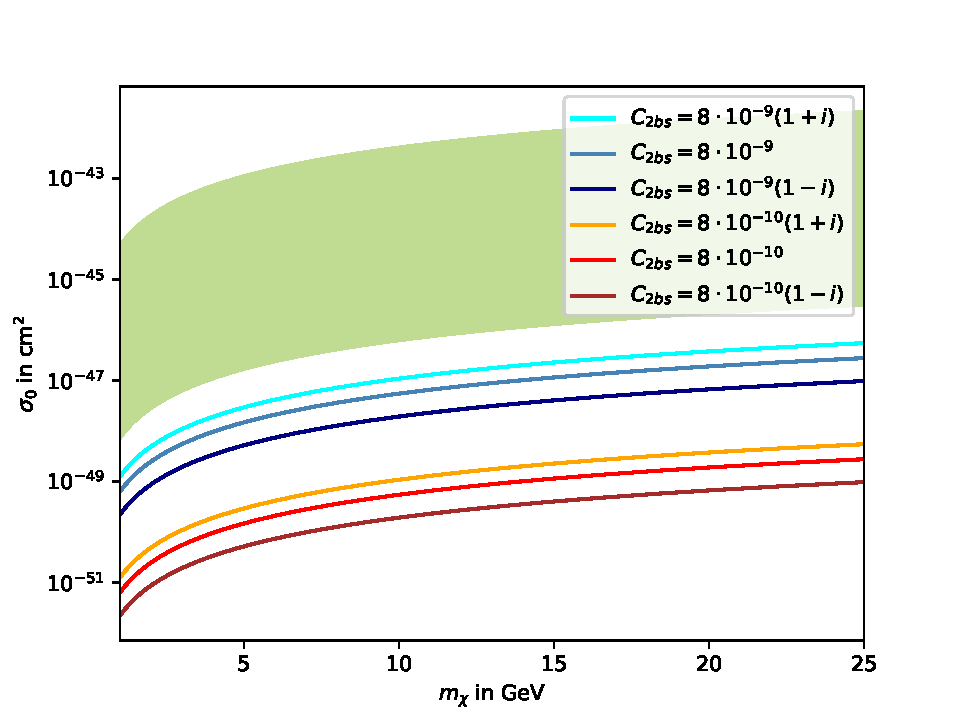
\includegraphics[width=\textwidth]{content/graphics/Allgemein11.pdf}
		\caption{$q_l=q_\chi=1$}
		\label{fig:Allg11}
	\end{subfigure}
	\begin{subfigure}[]{0.8\textwidth}
		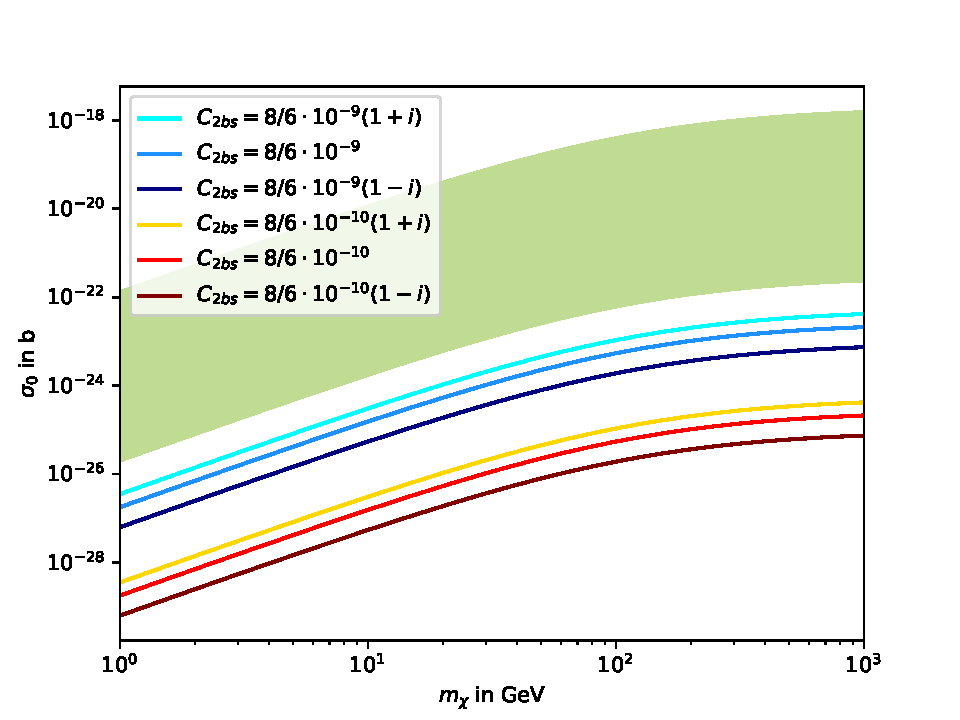
\includegraphics[width=\textwidth]{content/graphics/Allgemein116.pdf}
		\caption{$q_l=1,q_\chi=\sfrac{1}{6}$}
		\label{fig:Allg116}
	\end{subfigure}
	\caption{The shaded green area represents $\sigma_{0,\text{loop}}$ with the bounds in \eqref{eq:BoundBS}. The coloured lines show $\sigma_{0,\text{tree}}$ for different values of $C_{2bs}$ (in $\si{\giga\electronvolt}^{-2}$).}
	\label{fig:Allgemein}
\end{figure}

\begin{figure}
	\centering
	\begin{subfigure}[]{0.8\textwidth}
		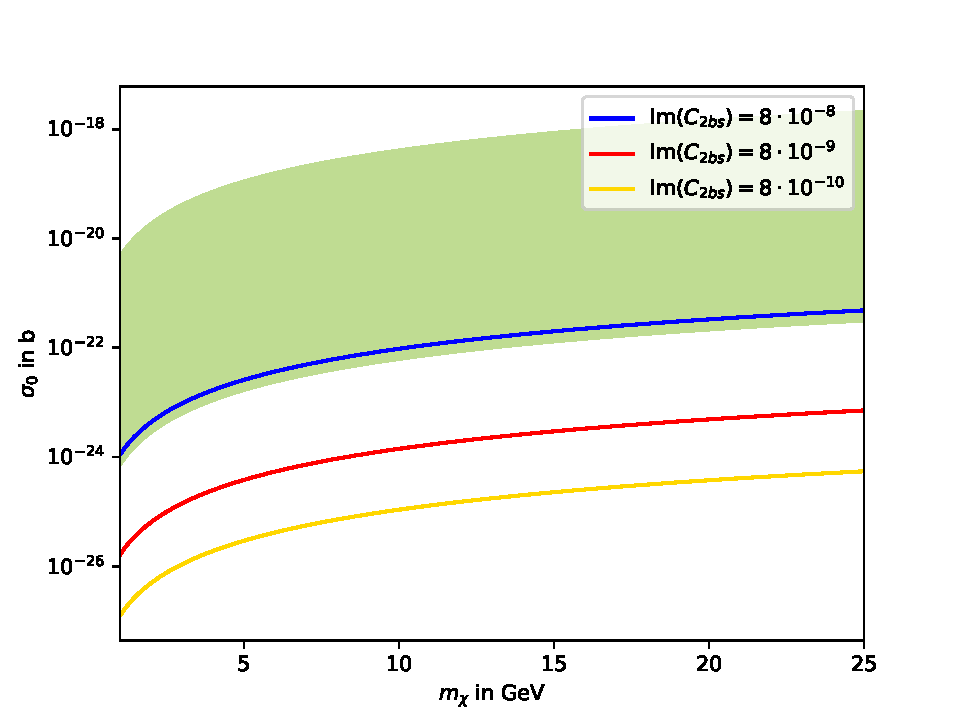
\includegraphics[width=\textwidth]{content/graphics/Im11.pdf}
		\caption{$q_l=q_\chi=1$}
		\label{fig:Im11}
	\end{subfigure}
	\begin{subfigure}[]{0.8\textwidth}
		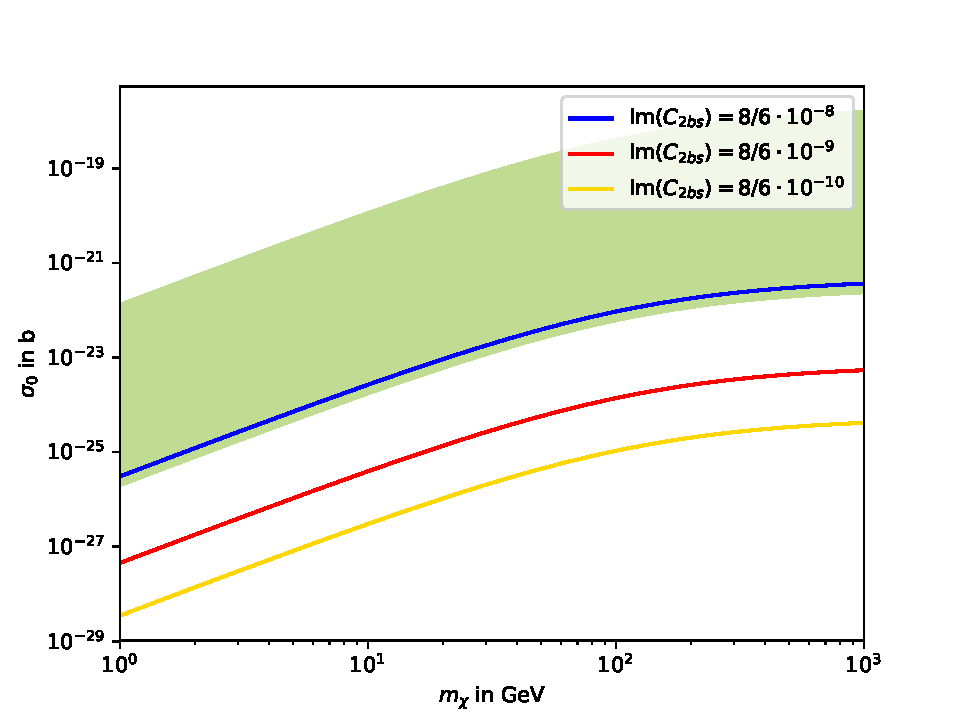
\includegraphics[width=\textwidth]{content/graphics/Im116.pdf}
		\caption{$q_l=1,q_\chi=\sfrac{1}{6}$}
		\label{fig:Im116}
	\end{subfigure}
	\caption{Like \ref{fig:Allgemein}, but the real part of $C_{2bs}$ is fixed at $\SI{8e-10}{\giga\electronvolt}^{-2}$ and only $\text{Im}(C_{2bs})$ is varied.}
	\label{fig:Im}
\end{figure}

\begin{figure}
	\centering
	\begin{subfigure}[]{0.8\textwidth}
		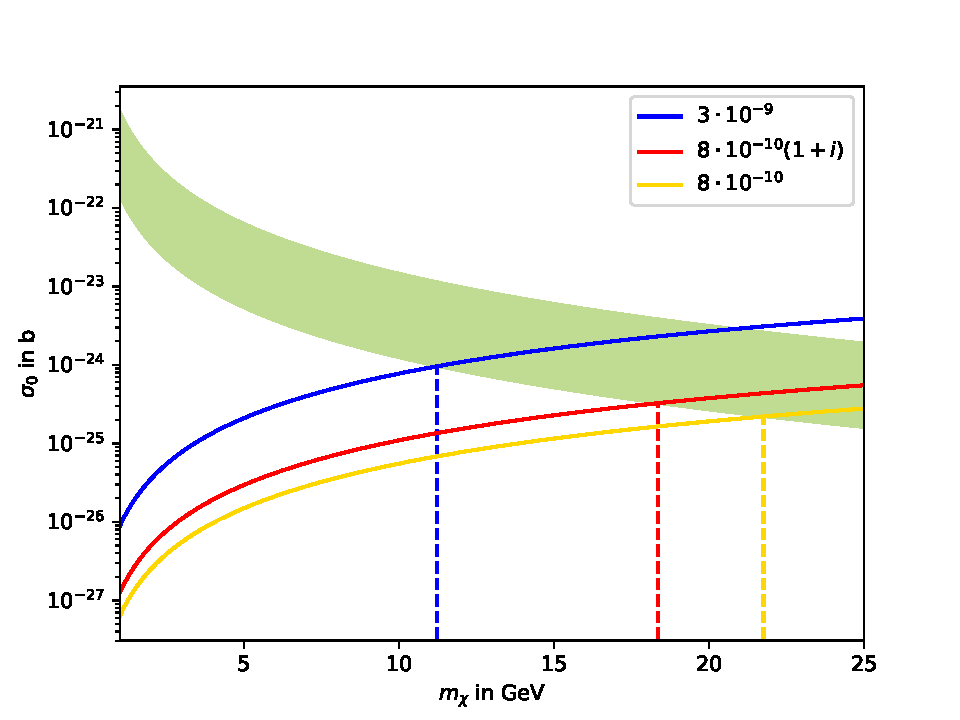
\includegraphics[width=\textwidth]{content/graphics/Relic11.pdf}
		\caption{$q_l=q_\chi=1,g'=\SI{2e-3}{}$}
		\label{fig:Relic11}
	\end{subfigure}
	\begin{subfigure}[]{0.8\textwidth}
		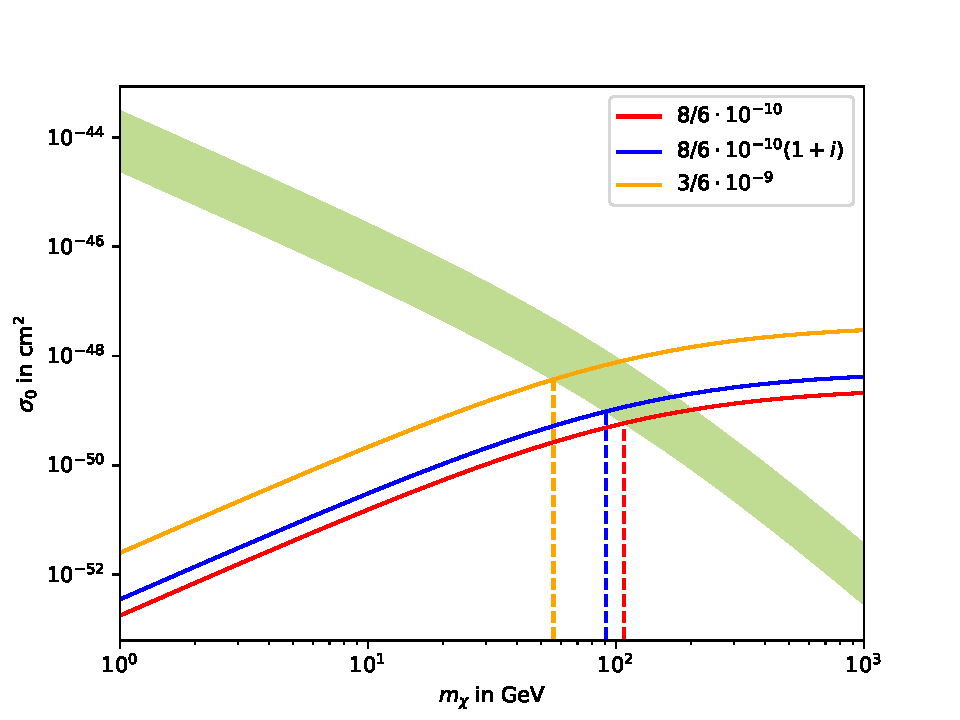
\includegraphics[width=\textwidth]{content/graphics/Relic116.pdf}
		\caption{$q_l=1,q_\chi=\sfrac{1}{6},g'=\SI{e-2}{}$}
		\label{fig:Relic116}
	\end{subfigure}
	\caption{The shaded green area represents the loop cross section $\sigma_{0,\text{loop}}$ at fixed coupling constant $g'$ and $m_{Z'} = 2m_\chi$ with a $\pm\SI{30}{\%}$ tolerance.}
	\label{fig:Relic}
\end{figure}


To make a long story short, if we respect the given bounds from the $B\rightarrow K\bar{l}l$ anomalies, we cannot find any parameter configuration for which the flavour mixing becomes relevant. So, Altmannshofer et. al. correctly neglect quark flavour mixing in the nucleus. However, the set-up presented in chapter \ref{sec:formalism} is universal and may, for example, be applied in the future to check whether ignoring flavour mixing was right in other new physics propositions.
%\chapter{Conclusion}
%\input{content/6_Conclusion.tex}

\appendix
% Hier beginnt der Anhang, nummeriert in lateinischen Buchstaben


\todos
\cleardoublepage
\backmatter
\printbibliography

\cleardoublepage
\thispagestyle{empty}
\section*{Eidesstattliche Versicherung}
Ich versichere hiermit an Eides statt, dass ich die vorliegende Abschlussarbeit mit dem Titel \enquote{\thetitle} selbstständig und ohne unzulässige fremde Hilfe erbracht habe.
Ich habe keine anderen als die angegebenen Quellen und Hilfsmittel benutzt, sowie wörtliche und sinngemäße Zitate kenntlich gemacht. 
Die Arbeit hat in gleicher oder ähnlicher Form noch keiner Prüfungsbehörde vorgelegen.

\vspace*{1cm}\noindent
\begin{center}
  \begin{tabular}{@{}p{0.4\textwidth}@{\hspace{0.15\textwidth}}p{0.4\textwidth}@{}}
  \rule{\linewidth}{0.25pt}& \rule{\linewidth}{0.25pt}\\
  Ort, Datum & Unterschrift
  \end{tabular}
\end{center}

\subsection*{Belehrung}
Wer vorsätzlich gegen eine die Täuschung über Prüfungsleistungen betreffende Regelung einer Hochschulprüfungsordnung verstößt, handelt ordnungswidrig.
Die Ordnungswidrigkeit kann mit einer Geldbuße von bis zu \SI[round-mode=places, round-precision=2]{50000}{€} geahndet werden. 
Zuständige Verwaltungsbehörde für die Verfolgung und Ahndung von Ordnungswidrigkeiten ist der Kanzler/die Kanzlerin der Technischen Universität Dortmund. 
Im Falle eines mehrfachen oder sonstigen schwerwiegenden Täuschungsversuches kann der Prüfling zudem exmatrikuliert werden (\S\,63 Abs. 5 Hochschulgesetz --HG--).

Die Abgabe einer falschen Versicherung an Eides statt wird mit Freiheitsstrafe bis zu 3 Jahren oder mit Geldstrafe bestraft.

Die Technische Universität Dortmund wird ggf.\ elektronische Vergleichswerkzeuge (wie z.\,B.\ die Software \enquote{turnitin}) zur Überprüfung von Ordnungswidrigkeiten in Prüfungsverfahren nutzen. \\[\baselineskip]

\noindent Die oben stehende Belehrung habe ich zur Kenntnis genommen.\\[1cm]
\begin{center}
\begin{tabular}{@{}p{0.4\textwidth}@{\hspace{0.15\textwidth}}p{0.4\textwidth}@{}}
\rule{\linewidth}{0.25pt}& \rule{\linewidth}{0.25pt}\\
Ort, Datum & Unterschrift
\end{tabular}
\end{center}

\end{document}
